\documentclass[11pt]{article}
\usepackage[a4paper, margin=1in]{geometry}

\usepackage[hidelinks]{hyperref}
\hypersetup{
	colorlinks=true,
	linkcolor=blue,
}
\usepackage{amsfonts, amsmath, amssymb, amsthm}
\usepackage{graphicx}
\usepackage{subfigure}
\usepackage{caption}
\usepackage{subcaption}
\usepackage{fancyhdr}



\begin{document}
	\begin{titlepage}
		\begin{center}
			\begin{figure}
				\centering
				
\includegraphics[scale=0.15]{images/IUST_Logo.jpg} \\
				\caption*{\textbf{School of Mathematics \& Computer Science}}
			\end{figure}
			\vspace*{0.5cm}
			\Huge{\textbf{Comparison of \\ Numerical Methods and PINNs \\ for the Schrödinger equation}}\\
			\vspace*{3cm}
			\large{\textbf{Mohsen Peykanro}}\\
			\large{\textbf{Ehsan Pichka}}\\
			\large{\textbf{Arshia Soleymani}}\\
			\vspace*{3cm}
			\large{\textbf{Advisor:}}\\
			\large{\textbf{Dr. Mahboubeh Molavi Arabshahi}}\\
			\vspace*{3cm}
			\today
		\end{center}
	\end{titlepage}
	
\section{Introduction}
\subsection{Background}
The Schrödinger equation is a partial differential equation in quantum mechanics that describes how the quantum state of a physical system change over time. This equation can handle the behavior of particles at the microscopic level. This equation have two forms that are based on times. The time-dependent Schrödinger equation describes the change of a system's wave function over time, while the time-independent version is used to determine stationary states and energy levels.

In most cases, you cant solve the equation so the exact analytical solutions are not available, especially for complex potentials or higher-dimensional systems. As a result, numerical methods play a crucial role in approximating solutions. The solution to the Schrödinger equation is called the wave function that provides information about the probability distribution of a particle's position and momentum. We mostly are going to survey Classical numerical approaches and Physics-Informed Neural Networks (PINNs) in this article.

The Classical numerical approaches such as the finite difference method (FDM) and finite element method (FEM) have been widely used for solving partial differential equations like Schrödinger equation. These methods rely on discretization of the domain and typically require careful handling of stability, convergence, and computational cost. On the other hand in recent years, PINNs have appeard as a modern approach for solving differential equations. PINNs merge the physical laws directly into the loss function of a neural network, so the solution will be approximated without discretization of the domain. This makes PINNs usefull for complex and high-dimensional problems.

\subsection{Objective of the Study}
The main objective of this paper is to compare classical numerical methods and Physics-Informed Neural Networks in solving the Schrödinger equation. Despite the growing interest in PINNs, we are not quite sure that how they compare to classical numerical methods in terms of accuracy, efficiency, and stability. A systematic comparison is necessary to evaluate their strengths and limitations.

\section{Mathematical Formulation}
\subsection{Early-Stage Quantum Theory}
The Schrödinger equation is a direct consequence of the discovery of quanta in the early 20th century. Its origins lie in the energy quanta hypothesis proposed by Max Planck in 1900 and the photon hypothesis by Albert Einstein in 1905, which established that energy and momentum are quantized.
\begin{equation}  \label{eq:1905}
	E = h \nu = \hbar \omega
\end{equation} 
where $E$ denotes energy, $h$ is the Plnack constant ($6.626 \times 10^{-34} \,\text{J·s}$) and $\nu$ is frequency of light. so now we can define the reduced Planck constant as $\hbar = \frac{h}{2 \pi}$ and $\omega = 2 \pi \nu$ as angular frequency. 
Later on, Einstein in 1917 concluded that momentum of light quantum $p$ is:
\begin{equation}  \label{eq:1917}
	 p = \frac{E}{c} = \frac{\hbar \omega}{c} = \hbar k 
\end{equation}
$k$ is called wavenumber and is defind as $ k = 2 \pi \lambda$, where $\lambda$ is wavelength of light in vacuum.

In 1923, Arthur Compton conducted experiments investigating how incident X-ray beams were scattered by matter, such as graphite and copper. He discovered a systematic redshift (an increase in wavelength) in the scattered X-rays and they call it Compton effect. Moreover he found that the shift in wavelengths depended only on the scattering angle regardless of quality of material of a scatterer. 
\begin{equation}
	\Delta \lambda = \frac{h}{m_e c} (1 - \cos \theta) 
\end{equation} 
where $\Delta \lambda$ means a Shift in wave length of scatterd beam, $m_e$ is a rest mass of an electron (mass that is independent of the motion of the particle) and $\theta$ is a scatering angle of the beam. The constant $\frac{h}{m_e c} $ is defined as the electron Compton wavelength ( $\lambda_e$) approximately $ 2.426 \times 10^{-12} $ meters.

\begin{figure}[h!]
	\centering
	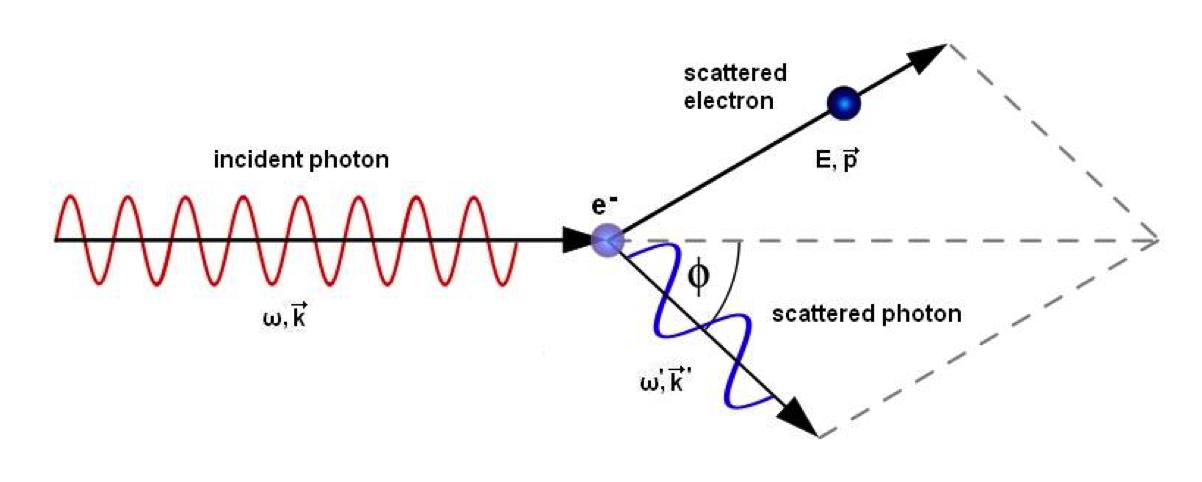
\includegraphics[height=5cm]{images/Fig5}
	\caption{Compton effect: scattering of a photon on a resting electron}
\end{figure}


In 1924, Louis de Broglie Encouraged by the success of Einstein and Compton in proving that waves (light) could behave like particles and theorized that the reverse must also be true, in other word matter particles must possess a wave nature. De Broglie essentially reversed the relationship of (\ref{eq:1905}) and (\ref{eq:1917}) such that
\begin{equation}
	\omega = \frac{E}{\hbar}, \quad k = \frac{p}{\hbar} \quad \text{or} \quad \lambda = \frac{h}{p}
\end{equation}
where $p$ equals $|p|$ and $\lambda$ is a wavelength of a corpuscular beam(a directional stream of tiny particles). this is called de Broglie wavelength (matter wave). this equation implies that if we are able to determine the wavelength of the corpuscular beam experimentally, we can decide a magnitude of momentum accordingly.

For a matter wave, the phase velocity $v_p$ is shown to be greater than $c$, while the group velocity $v_g$, which represents the propagation velocity of a wave packet (and thus the particle's velocity), is less than $c$. Their relationship is defined by $v_p v_g = c^2$. Therefore, a particle velocity must not exceed $c$.
\begin{figure}[h!]
	\centering
	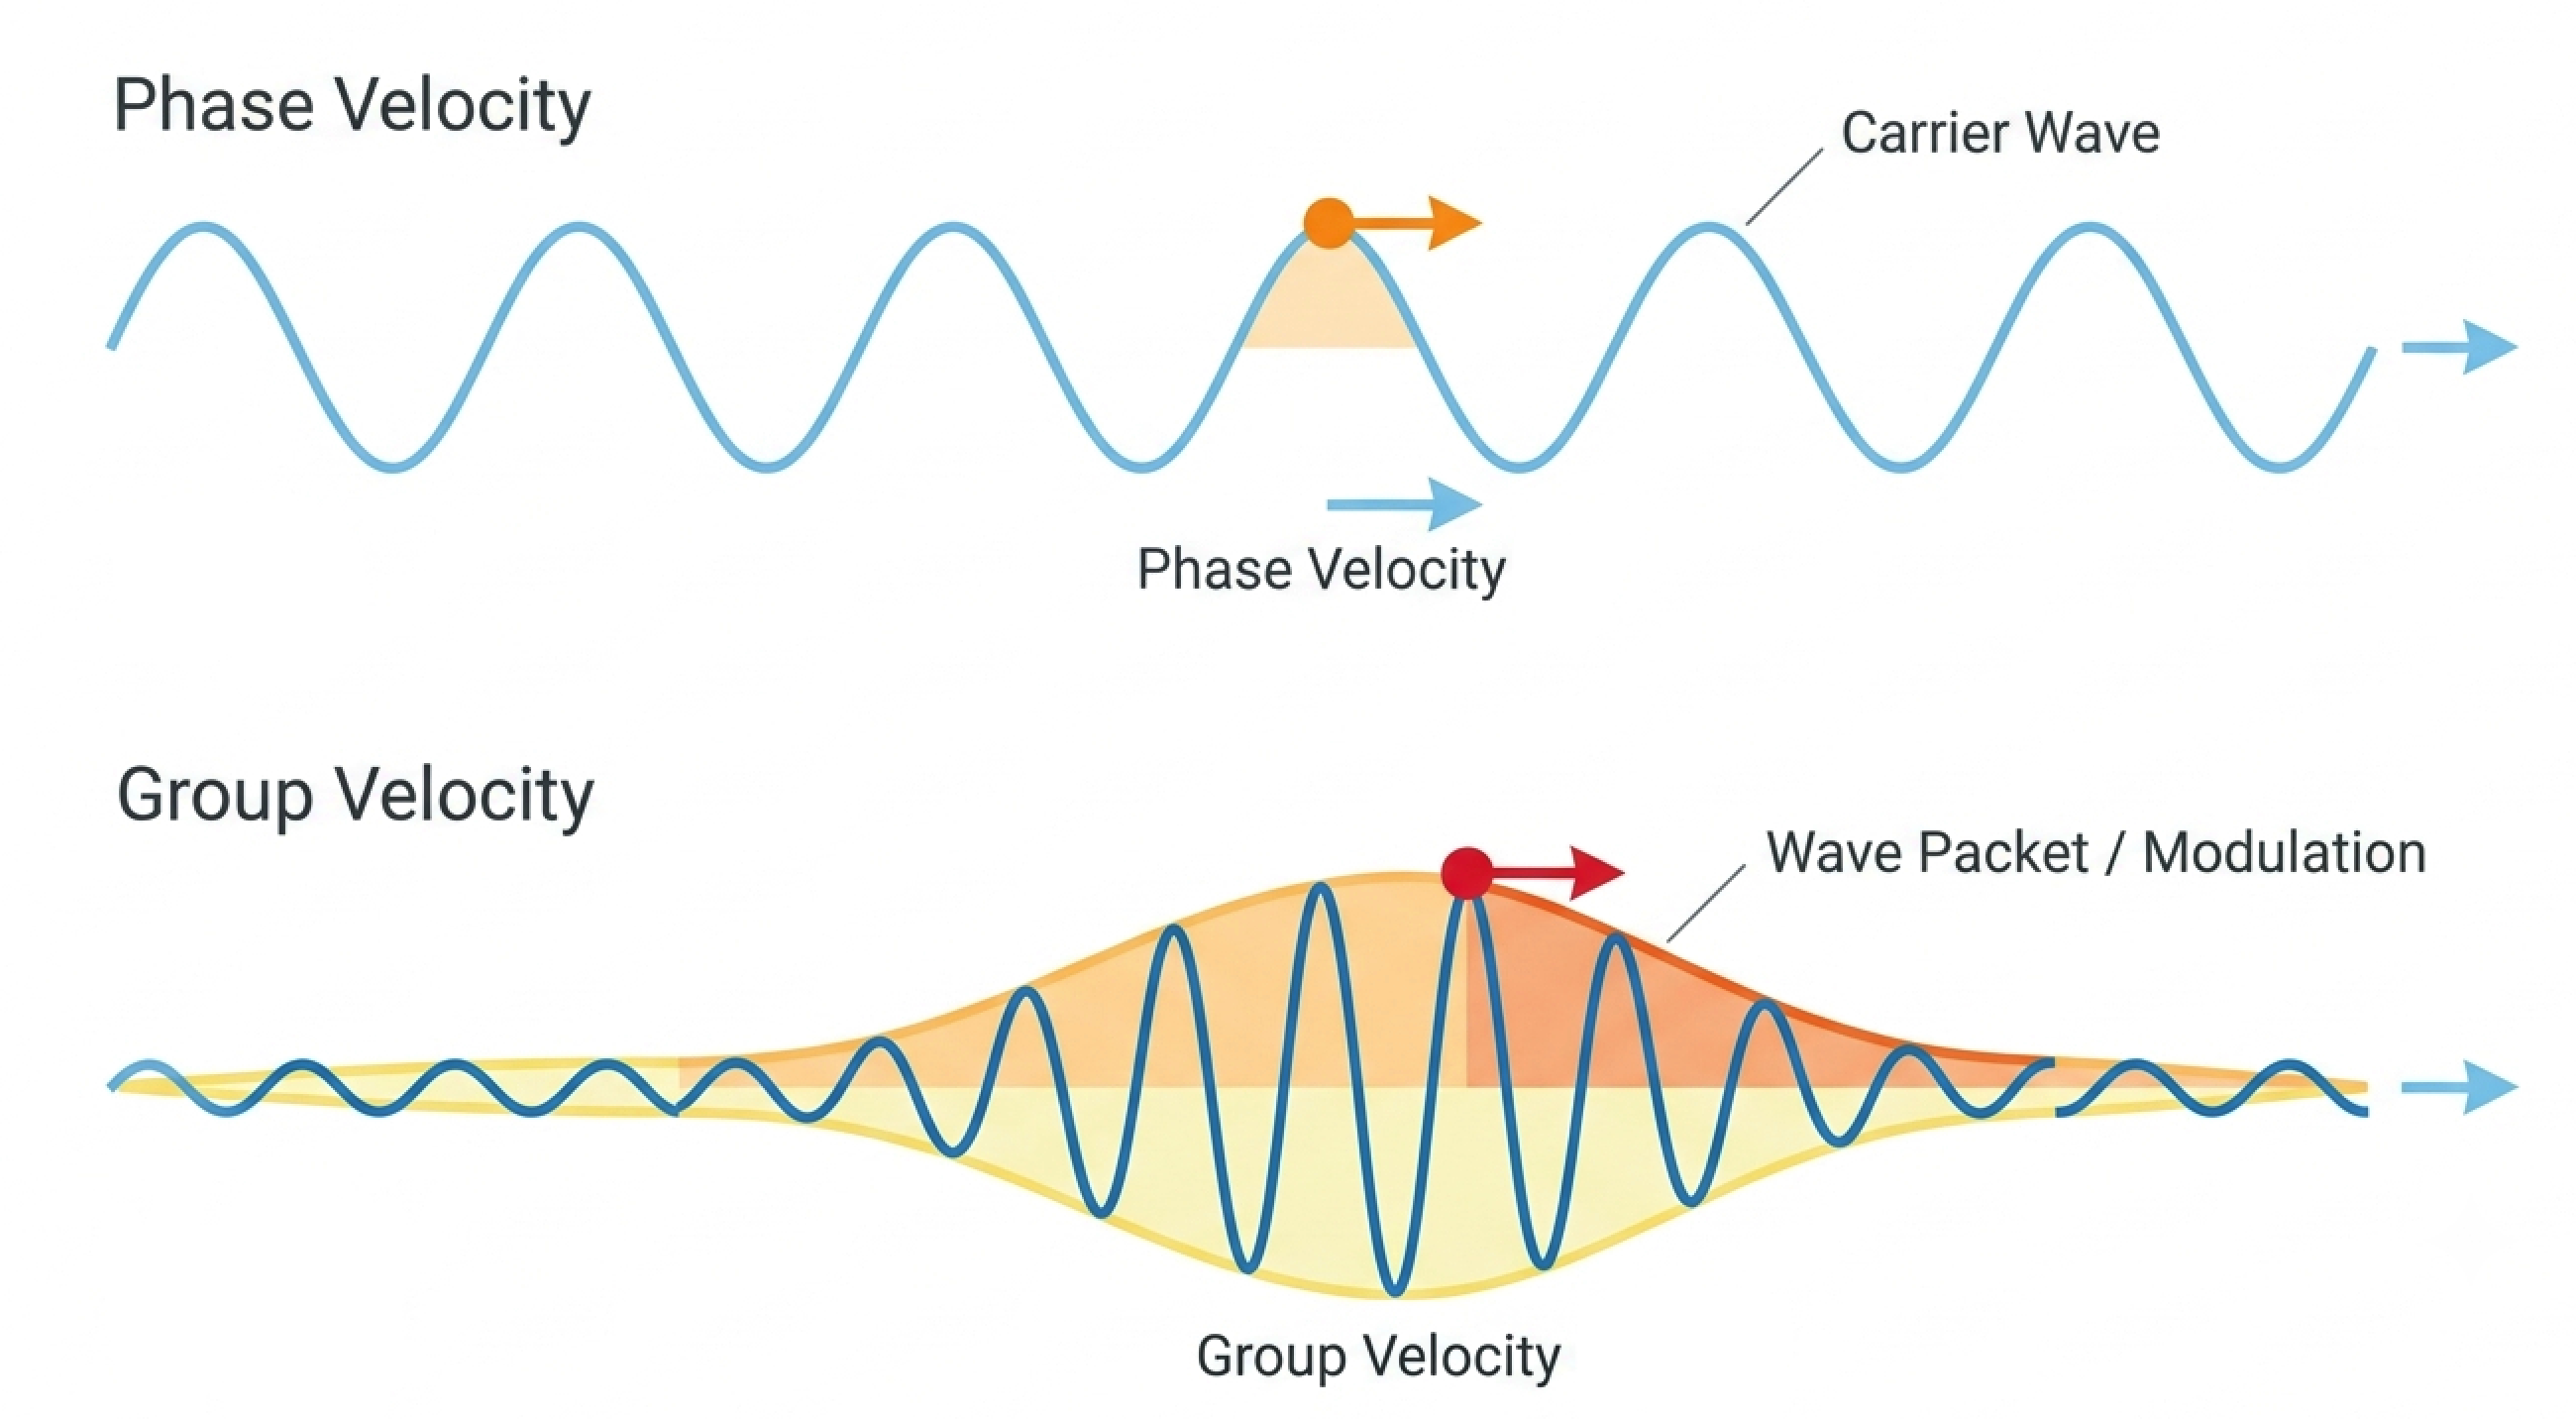
\includegraphics[height=5cm]{images/Fig2}
	\caption{Phase velocity vs Group velocity}
\end{figure}

\subsection{Time-Dependent Schrödinger Equation}
The derivation starts with the standard wave equation 
\begin{equation}
	\nabla^2 \Psi = \frac{1}{v^2} \frac{\partial^2 \Psi}{\partial t^2}
\end{equation}
where $\Psi$ is an arbitrary function of a physical quantity relevant to propagation of a wave(shape of a wave), $v$ is a phase velocity of wave, $ \nabla^2$ is called Laplacian and is defined as
\begin{equation}
	\nabla^2 \equiv \frac{\partial^2}{\partial x^2} + \frac{\partial^2}{\partial y^2} + \frac{\partial^2}{\partial z^2}
\end{equation}

\begin{figure}[h!]
	\centering
	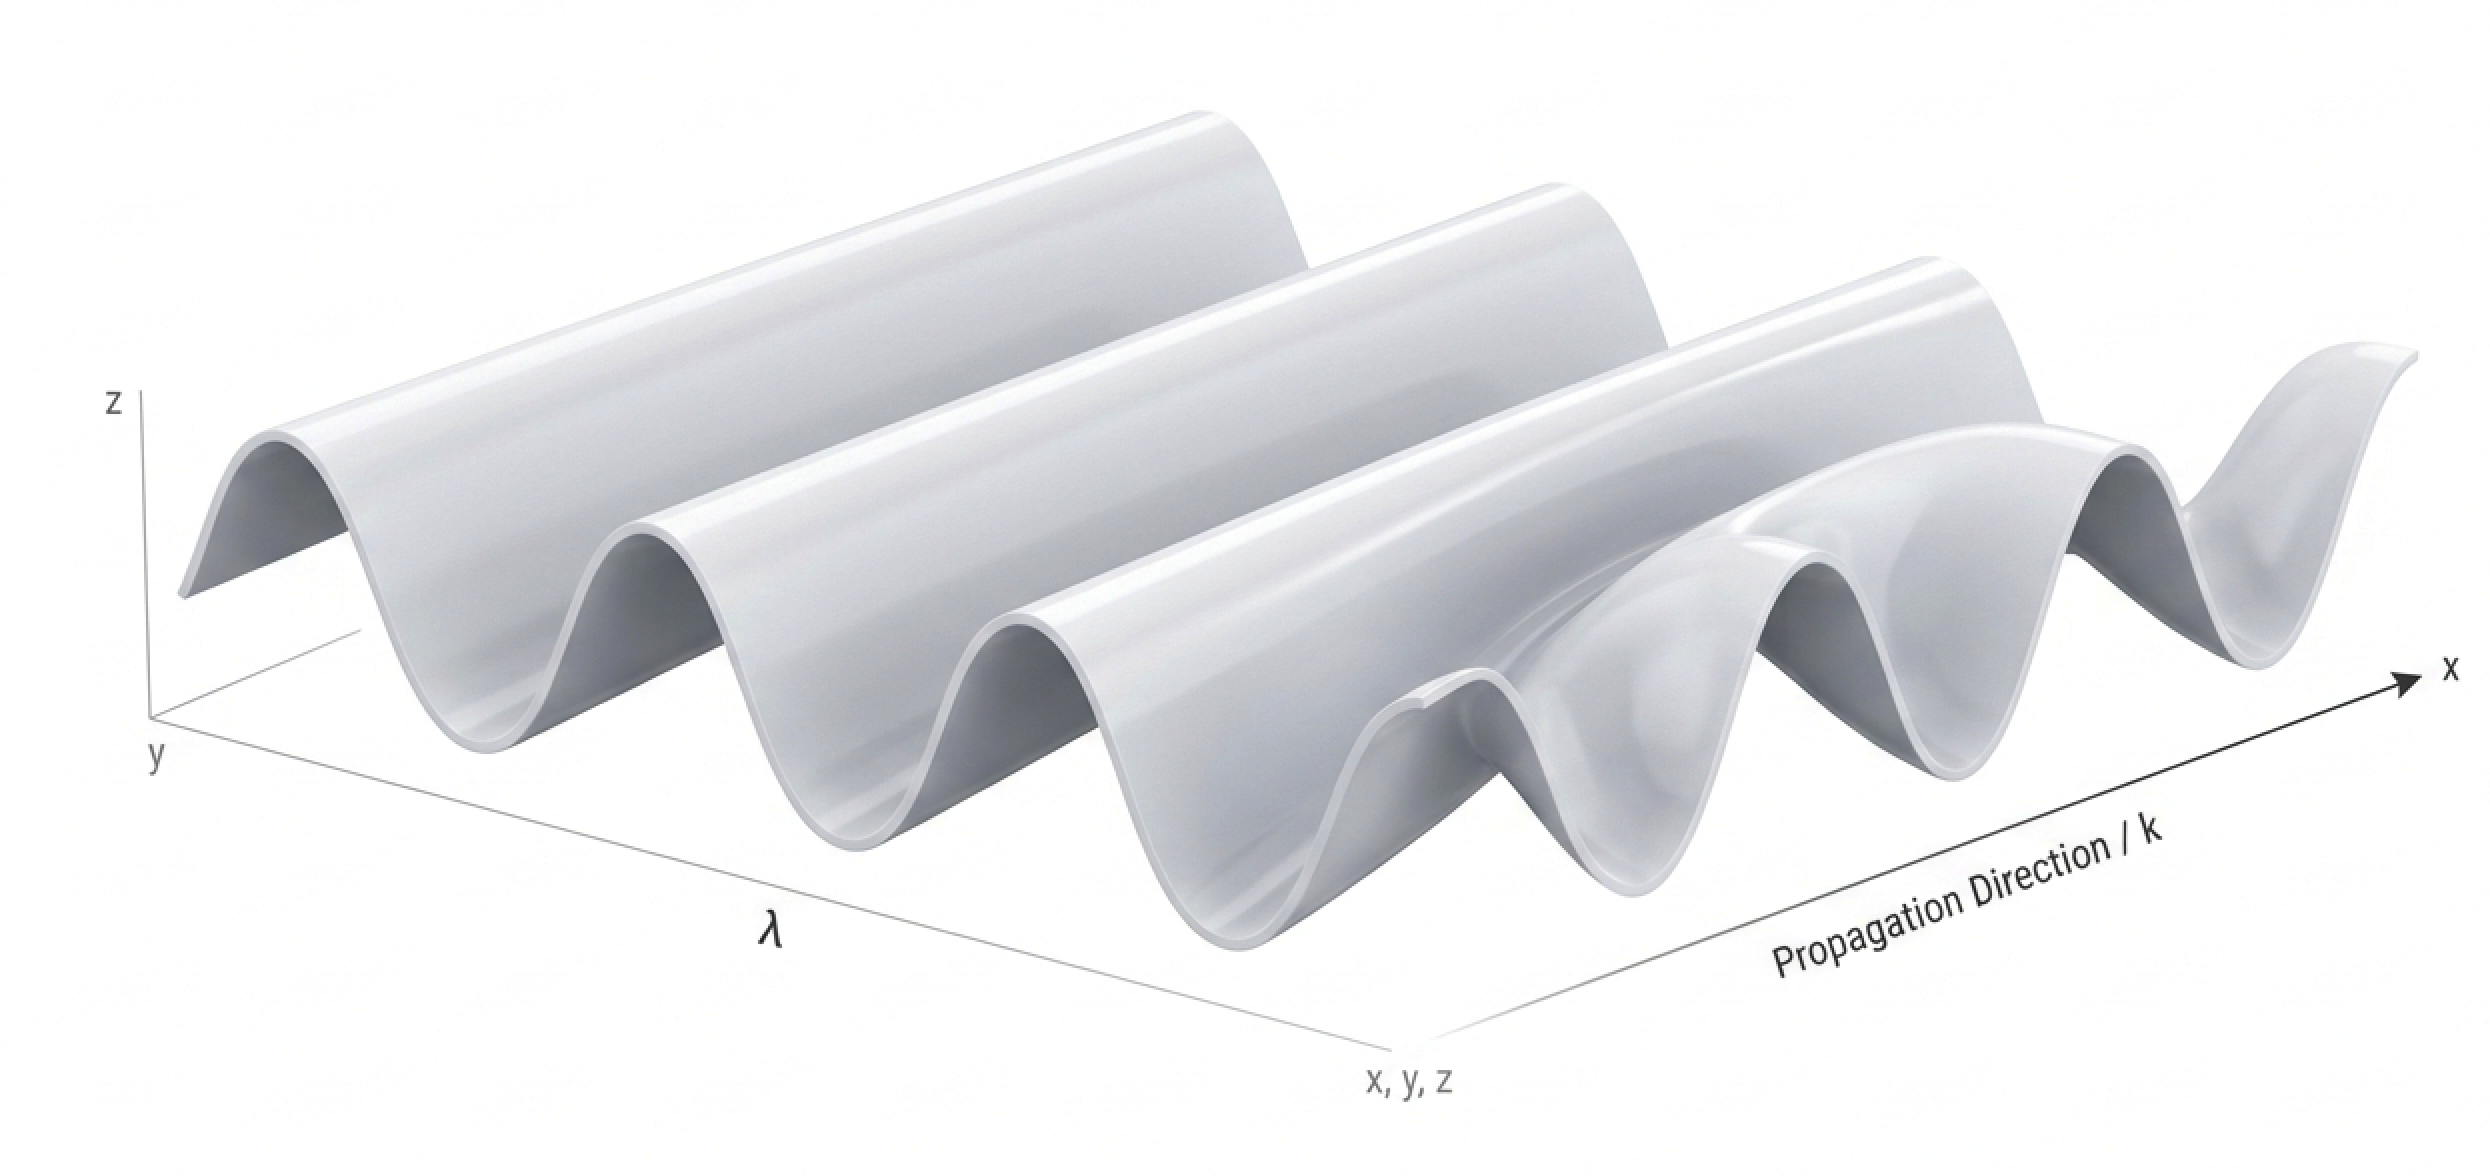
\includegraphics[width=7.5cm]{images/Fig3}
	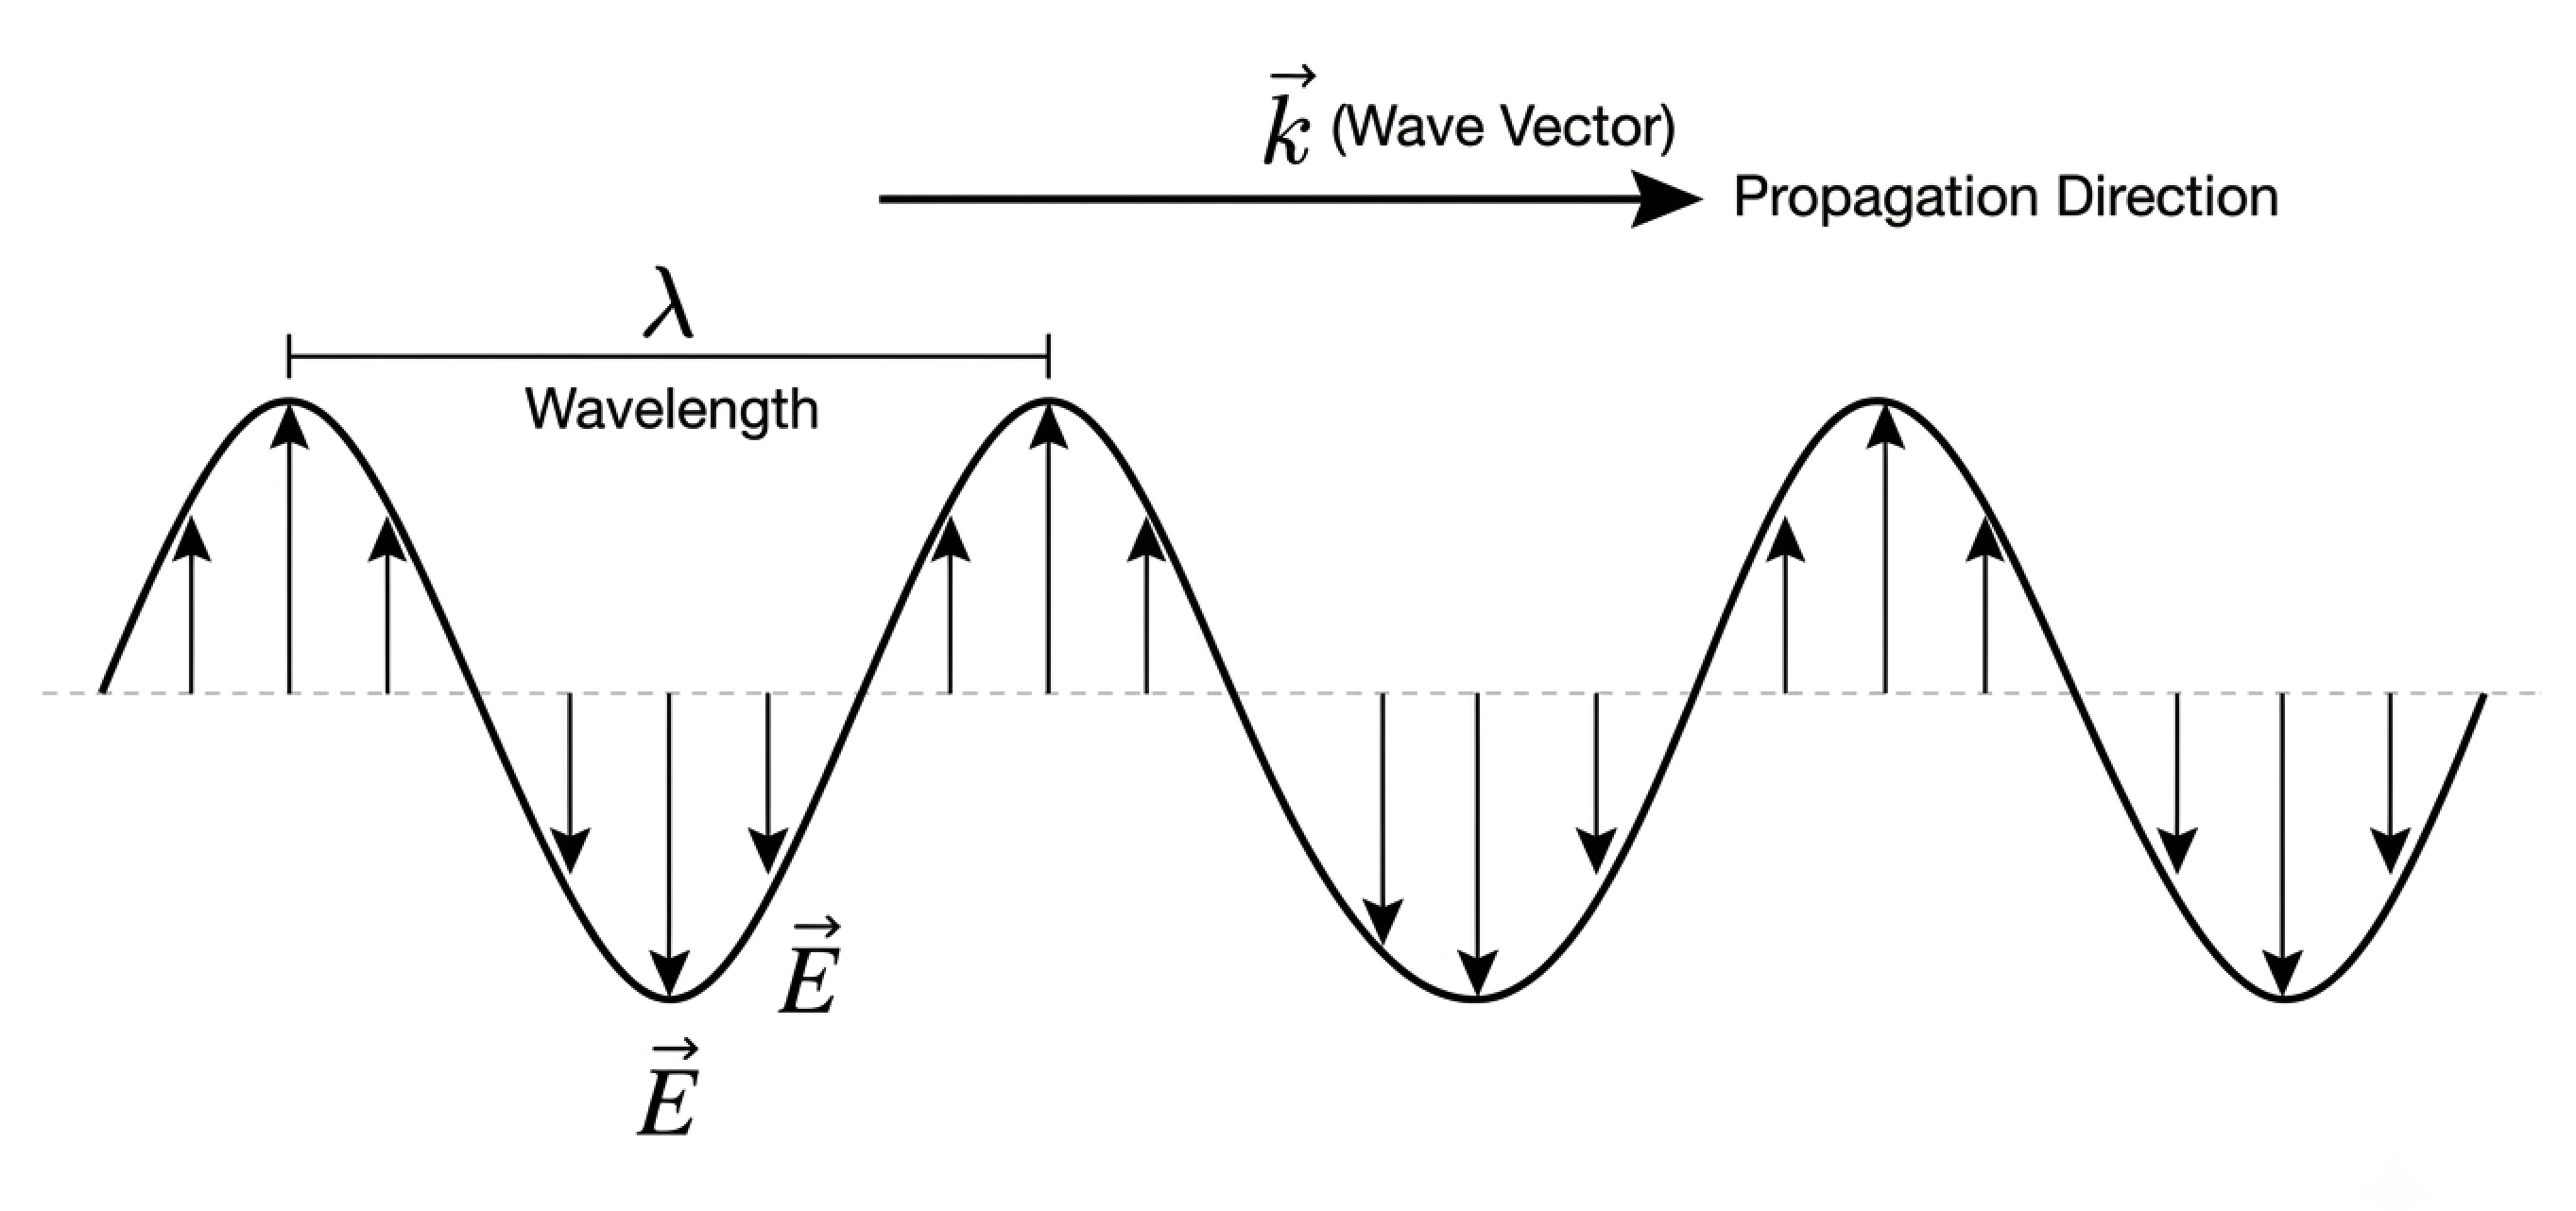
\includegraphics[width=7.5cm]{images/Fig4}
	\caption{Plane waves in two and three dimensions}
\end{figure}

One of the special solutions for wave equation is called a plane wave and its expressed as
\begin{equation}
	\Psi = \Psi_0 e^{i(k \cdot x - \omega t)} = \Psi_0 [ \cos (k \cdot x - \omega t) + i \sin (k \cdot x - \omega t) ]
\end{equation}
where $x$ denotes a position vector of a three-dimensional Cartesian coordinate. By applying de Broglie and Einstein’s relations, this is converted into a matter wave representing a particle:
\begin{equation} \label{eq:8}
	\Psi = \Psi_0 e^{i(\frac{p}{h} \cdot x - \frac{E}{h} t)}, \quad 
	p = \begin{pmatrix} e_1 \; e_2 \; e_3 \end{pmatrix} \begin{pmatrix} p_x \\ p_y \\ p_z \end{pmatrix}
\end{equation}
taking partial differentiation with respect to $x$ we obtain
\begin{equation}
	\frac{\partial \Psi}{\partial x} = \frac{i}{\hbar} p_x \Psi_0 e^{i(\frac{p}{h} \cdot x - \frac{E}{h} t)} = \frac{i}{\hbar} p_x \Psi \quad \Rightarrow \quad
	\frac{\hbar}{i} \frac{\partial \Psi}{\partial x} = p_x \Psi
\end{equation}
Similarly we have
\begin{equation}
	\frac{\hbar}{i} \frac{\partial \Psi}{\partial y} = p_y \Psi \quad \text{and} \quad \frac{\hbar}{i} \frac{\partial \Psi}{\partial z} = p_z \Psi
\end{equation}
Taking partial differentiation once more 
\begin{equation}
	\frac{\partial^2 \Psi}{\partial x^2} = (\frac{i}{\hbar} p_x)^2 \Psi_0 e^{i(\frac{p}{h} \cdot x - \frac{E}{h} t)} = - \frac{1}{\hbar^2} p_x^2 \Psi \quad \Rightarrow \quad
	- \hbar^2 \frac{\partial^2 \Psi}{\partial x^2} = p_x^2 \Psi
\end{equation}
Similarly we have
\begin{equation}
	- \hbar^2 \frac{\partial^2 \Psi}{\partial y^2} = p_y^2 \Psi \quad \text{and} \quad - \hbar^2 \frac{\partial^2 \Psi}{\partial z^2} = p_z^2 \Psi
\end{equation}
So if we summing both sides of these 3 equation and then dividing by $2m$ ($m$ is the mass of a particle), we have
\begin{equation} \label{eq:13}
	- \frac{\hbar ^ 2}{2m} \nabla^2 \Psi - \frac{p^2}{2m} \Psi
\end{equation}

Now lets get back to equation (\ref{eq:8}) and this time taking partial differentiation with respect to $t$, we obtain
\begin{equation} \label{eq:14}
	\frac{\partial \Psi }{\partial t} = - \frac{i}{\hbar} E \Psi_0 e^{i(\frac{p}{h} \cdot x - \frac{E}{h} t)} = - \frac{i}{\hbar} E \Psi \quad \Rightarrow \quad 
	i \hbar \frac{\partial}{\partial t} = E \Psi
\end{equation}
If we subtract (\ref{eq:13}) and (\ref{eq:14}) we get
\begin{equation} \label{eq:15}
	i \hbar \frac{\partial \Psi}{\partial t} + \frac{\hbar ^2}{2m} \nabla^2 \Psi = (E - \frac{p^2}{2m}) \Psi
\end{equation}
Comparing these equations we find out that momentum $p$ becomes the operator $ \frac{\hbar}{i} \nabla$ and energy $E$ becomes the operator $ i \hbar \frac{\partial}{\partial t}$. Now if we substituting these operators into the classical energy conservation relation (Total energy = Kinetic energy + Potential energy) we have
\begin{equation}
	E = \frac{p^2}{2m} + V
\end{equation}
So now lets rewrite the equation (\ref{eq:15})
\begin{equation} \label{eq:TDSE}
	i \hbar \frac{\partial \Psi}{\partial t} + \frac{\hbar ^ 2}{2m} \nabla^2 \Psi = V \Psi \quad \Rightarrow \quad
	(- \frac{\hbar ^ 2}{2m} \nabla^2 + V) \Psi = i \hbar \frac{\partial \Psi}{\partial t}
\end{equation}
This is the Time-Dependent Schrödinger Equation (TDSE), a fundamental equation of quantum mechanics. 

If we defind a following Hamiltonian operator $H$ (the sum of two components, the kinetic energy and the potential energy of a quantum system) as 
\begin{equation}
	H \equiv - \frac{\hbar^2}{2m} \nabla^2 + V 
\end{equation}
Then we have a shorthand representation such that
\begin{equation}
	H \Psi = i \hbar \frac{\partial \Psi}{\partial t}
\end{equation}
Since we want to associate the wave function with a single particle, it is reasonable to require the probability to find the electron anywhere in space to be exactly equal to one. Since this may not be the case for all $\Psi$, we introduce a normalization condition:
\begin{equation}
	\int_{- \infty}^{\infty} | \Psi (x,t) |^2 dx = 1
\end{equation}
The normalization thus imposes a condition on the wave function, the wave function must be a square integrable function.

\subsection{Time-Independent Schrödinger Equation}
In (\ref{eq:TDSE}) $\Psi$ is a function of $x$ and $t$. Suppose that a potential $V$ depends only upon $x$ and seperation of variables can be done with $\Psi$ function ($\Psi(x,t) = \phi(x) \xi(t)$). By substituting these functions into the Time-Dependent Schrödinger Equation, we have
\begin{equation}
	- \frac{\hbar^2}{2m} \nabla^2 \phi(x) \xi(t) + V(x) \phi(x) \xi(t) = i \hbar \phi(x) \frac{\partial \xi(t)}{\partial t}
\end{equation}
Now we will dividing the entire equation by $\phi(x) \xi(t)$
\begin{equation}
	\frac{- \frac{\hbar^2}{2m} \nabla^2 \phi(x)}{\phi(x)} + V(x)  = \frac{i \hbar \frac{\partial \xi(t)}{\partial t}}{\xi(t)}
\end{equation}
Since now the left hand side is only dependent on $x$ and the right hand side only on $t$, both sides must be equal to a constant, which is defined as the total energy$E$, and we can now solve each side independently
\begin{equation}\label{eq:TISE}
	H \phi(x) = E \phi(x)
\end{equation}
\begin{equation}
	\begin{aligned}
	& i \hbar \frac{\partial \xi(t)}{\partial t} = E \, \xi(t) 
	\quad \Rightarrow \quad \frac{d \xi(t)}{\xi(t)} = \frac{E}{i \hbar} \, dt 
	\quad \Rightarrow \quad \int \frac{d \xi}{\xi} = \frac{E}{i \hbar} \int dt \\
	& \quad \Rightarrow \quad \ln \frac{\xi(t)}{\xi(0)} = \frac{E t}{i \hbar} 
	\quad \Rightarrow \quad \xi(t) = \xi(0)\, \exp\!\left(-\frac{iEt}{\hbar}\right)
\end{aligned}
\end{equation}
The Time-Independent Schrödinger Equation (TISE)(\ref{eq:TISE}), is an eigenvalue problem where $E$ represents the energy eigenvalues and $\phi(x)$ represents the eigenfunctions (or stationary states) of the Hamiltonian operator. After solving the problem, we get a solution
\begin{equation}
	\Psi(x,t) = \phi(x) \exp\!\left(-\frac{iEt}{\hbar}\right)
\end{equation}

\section{Classical numerical methods for Schrödinger equation}
Classical numerical methods for solving the Schrödinger equation work by turning a continuous problem into a form that can be handled by a computer. Some common methods include finite difference and finite element methods, which divide space into small pieces and approximate derivatives. Spectral methods, such as Fourier, Chebyshev, and B-spline methods, instead represent the solution using combinations of known functions. Other useful approaches include the split-step Fourier method and the Crank–Nicolson method, which are often used to simulate how a system changes over time. Monte Carlo methods can also be used, especially for more complex or higher-dimensional problems.

For time-dependent Schrödinger equations, methods like Crank–Nicolson, implicit–explicit schemes, and operator splitting are popular because they are stable and work well for step-by-step time evolution. On the other hand, time-independent problems are usually solved using matrix diagonalization, variational methods, or Monte Carlo techniques to find energy levels and corresponding wave functions.

\subsection{Finite Difference Methods}
Finite Difference Methods (FDM) are numerical techniques used to approximate solutions to differential equations by discretizing the equations in both time and space. The continuous derivatives in the equations are replaced with finite difference approximations, which transform the problem into a system of algebraic equations that can be solved computationally. FDM is widely used to solve both time-dependent and time-independent forms of the Schrödinger equation.

\subsubsection{Discretizing the Domain}
Discretizing the domain transforms the continuous space and time where the wave function $\Psi (x,t)$ exists into a finite set of specific points called a mesh or grid, because computers cannot handle an infinite continuum of points.

The spatial domain is divided into equally spaced grid points defined as 
\begin{equation}
	x_j = j \Delta x \; ; \quad j = 0, 1, 2, \cdots , N
\end{equation}
where $\Delta x$ is the spatial step size and determines the resolution of the numerical approximation, with smaller values generally leading to higher accuracy at the expence of increased computaional cost.

Similarly, the time domain is divided into discrete time levels. The time points are defined as 
\begin{equation}
	t_n = n \Delta t \; ; \quad n = 0, 1, 2, \cdots
\end{equation}
where $\Delta t$ is the time step size and used to evolve the solution from one moment to the next.

After discretization, the continuous wave function $\Psi (x,t)$ is replaced by discrete values evaluated at the grid points. The value of the wave function at position $x_j$ and time $t_n$ is denoted by
\begin{equation}
	\Psi_j^n \approx \Psi (x_j, t_n)
\end{equation}
At any time step $n$ the entire spatial state can be treated as a vector 
\begin{equation}
	U^n = \begin{pmatrix} \Psi_0^n \\ \Psi_1^n \\ \vdots \\ \Psi_N^n \end{pmatrix}
\end{equation}
which represents the numerical state of the system at that particular time.

\subsubsection{Approximating the Schrödinger Equation}
After discretizing the computational domain, the next step in the finite difference method is to approximate the derivatives appearing in the Schrödinger equation. Since numerical algorithms cannot directly evaluate continuous derivatives, these derivatives are replaced by algebraic expressions involving values of the wave function at neighboring grid points. This transformation converts the differential equation into a system of algebraic equations that can be solved using a computer.

The kinetic energy term in the Schrödinger equation contains the second spatial derivative of the wave function. A commonly used approximation is the second-order centered finite difference formula
\begin{equation}
	\frac{\partial^2 \Psi}{\partial x^2} \approx \frac{\Psi_{j+1}^n - 2 \Psi_j^n + \Psi_{j-1}^n}{\Delta x^2}
\end{equation}
This approximation is second-order accurate, meaning that the truncation error is proportional to $O(\Delta x^2)$. As a resault, reducing the grid spacing improves the accuracy of the numerical solution.

The time derivative of the wave function can also be approximated using finite differences. One of the simplest approximations is the forward difference scheme
\begin{equation}
	\frac{\partial \Psi }{\partial t} \approx \frac{\Psi_j^{n+1} - \Psi_j^n}{\Delta t}
\end{equation}
For improved accuracy, central difference approximations may be employed. In this case, the derivative is approximated by
\begin{equation}
	\frac{\partial \Psi }{\partial t} \approx \frac{\Psi_j^{n+1} - \Psi_j^{n-1}}{2 \Delta t}
\end{equation}

\subsubsection{Implementation Strategies}
After discretization and derivative approximation, the finite difference equations must be solved using an appropriate numerical strategy. Several implementation techniques have been developed depending on the type of Schrödinger equation being considered and the desired numerical properties, such as stability, efficiency, and accuracy.

\begin{itemize}
	\item 
	The Method of Lines (MoL):
\end{itemize}
In this method, only the spatial derivatives(the Laplacian) are discretized using finite differences, while the time variable remains continuous. As a result, the Schrödinger equation is transformed into a system of coupled ordinary differential equations (ODEs) where $\hbar = m = 1$
\begin{equation}
	 \frac{d \Psi}{dt} = \frac{i}{2} \left[ \frac{\Psi_{j+1}^n - 2 \Psi_j^n + \Psi_{j-1}^n}{\Delta x^2} \right] - i V \Psi(t) \quad \Rightarrow \quad
	 \frac{d \Psi}{dt} = S(\Psi)
\end{equation}
Time evolution is then performed using an explicit third-order Runge–Kutta (RK3) scheme:
\begin{equation}
	k_1 = \Delta t S(\Psi ^n), \quad 
	k_2 = \Delta t S(\Psi ^n + \frac{1}{2} k_1), \quad 
	k_3 = \Delta t S(\Psi ^n + \frac{1}{2} k_2)
\end{equation}
\begin{equation}
	\Psi^{n+1} = \Psi^n + \frac{1}{6} k_1 +  \frac{2}{3} k_2 + \frac{1}{6} k_3
\end{equation}

\begin{itemize}
	\item 
	Imaginary Time Evolution (Wick Rotation):
\end{itemize}
Imaginary Time Evolution is a numerical technique commonly used to compute the stationary states of the Schrödinger equation, particularly the ground state. The method is based on the substitution $\tau = it$ where $t$ is the real time and $\tau$ is the imaginary time. This transformation, often referred to as a Wick rotation, converts the time-dependent Schrödinger equation into a diffusion-type equation (a partial differential equation that describes how a physical quantity spreads or smooths out over time due to diffusion-like processes: $\frac{\partial u}{\partial t} = D \nabla^2 u$).
\begin{equation}
	\frac{\partial}{\partial t} = i \frac{\partial}{\partial \tau} \quad \Rightarrow \quad
	\frac{\partial \Psi}{\partial \tau} = \frac{\hbar}{2m} \nabla^2 \Psi - \frac{V}{\hbar} \Psi 
\end{equation}
Notice that this has the same structure as the diffusion equation. The Laplacian causes the wavefunction to become smoother over imaginary time, while the potential term acts as a source or sink.

If the initial wave function is expressed as a linear combination of the eigenfunctions of the Hamiltonian we have
\begin{equation}
	\Psi(x, \tau) = \sum_{n} c_n \phi_n (x) e^{-E_n \tau}
\end{equation}
where $\phi_n(x)$ are the eigenfunctions, $E_n$ are the corresponding energy eigenvalues, and $c_n$ are expansion coefficients, each component decays exponentially as the imaginary time increases. As $ \tau \to \infty $, $e^{-(E_n - E_0) \tau} \to 0$ for $n > 0$. so only the ground state remains $\Psi (\tau) \approx c_0 \phi_0 e^{E_0 \tau}$

\begin{itemize}
	\item 
	Boundary Management:
\end{itemize}
For a finite computational domain $\Omega = [a,b]$, Dirichlet boundary conditions impose homogeneous constraints on the wave function $\Psi(a,t) = \Psi(b,t) = 0$. his corresponds to an infinite potential barrier outside $\Omega$, i.e.
\begin{equation}
	V(x) = 
	\begin{cases} 
		V(x) & \text{if } x \in \Omega \\
		\infty & \text{if } x \notin \Omega 
	\end{cases}
\end{equation}
To prevent waves from reflecting off the grid edges back into the simulation, an imaginary potential $\mathfrak{Im}(V)$ is added to the Hamiltonian and modifies the continuity equation for probability density $\rho = \Psi \Psi^* = |\Psi|^2$. If $\mathfrak{Im}(V)$ is negative, it acts as a sink, causing the probability density to decay as it enters the sponge region.
\begin{equation}
	\frac{\partial \rho}{\partial t} + \nabla \cdot J = 2 \rho \mathfrak{Im}(V)
\end{equation}
A typical smooth absorber is constructed using a hyperbolic tangent profile:
\begin{equation}
	\mathfrak{Im}(V) = - \frac{1}{2} V_0 \left\{ 2 + \tanh \left( \frac{(r - r_c)}{\delta}  \right) - \tanh (\frac{r_c}{\delta}) \right\}
\end{equation}
 where $V_0$ is the depth of the well, $r_c$ is the radius where the sponge starts, and $\delta$ is the transition width

For unbounded domains (infinite space), non-local boundary conditions allow waves to exit the domain as if the grid were infinite. These conditions are non-local in time, meaning the value at the boundary at time $t$ depends on the history of the wave function at that point. For a potential $V_-$ outside the boundary at $x=0$, the boundary condition takes the form
\begin{equation}
	\partial_x \Psi(0,t) = \sqrt{\frac{2}{\pi}} e^{-i\pi/4} e^{-iV_- t} \frac{d}{dt} \int_0^t \frac{\Psi(0,\tau)e^{iV_- \tau}}{\sqrt{t-\tau}}\, d\tau.
\end{equation}

\subsection{Finite Element Methods}
The Finite Element Method (FEM) is a numerical technique that approximates the solution by dividing the domain into a collection of small subdomains called finite elements, and finding an approximate solution using locally defined basis functions. Unlike the Finite Difference Method (FDM), which approximates derivatives directly at discrete grid points, FEM transforms the governing differential equation into its weak (variational) form before discretization. This formulation provides greater flexibility for handling complex geometries, irregular meshes and variable material properties.

\subsubsection{Discretizing the Domain}
Domain discretization is the first step. Let $\Omega \subset \mathbb{R}^d$ where $d=1,2,3$ denote the domain. Such that
\begin{equation}
	\bar{\Omega} = \bigcup_{e=1}^{m} \Omega_e
\end{equation}
where $\Omega_e$ represents the $e$th finite element and $m$ is the total number of elements. The interiors of any two distinct elements satisfy $\Omega_i \bigcap \Omega_j = \emptyset \quad i \neq j$ ensuring that the mesh completely covers the computational domain without overlap.  In 1D, elements are intervals $[ x_j, x_{j+1}]$, in 2D they are typically triangles or quadrilaterals and in 3D they are tetrahedra or hexahedra (bricks). Elements are interconnected at a finite number $N$ of nodal points $ \{ x_k \}_{k = 1}^N$ situated on their boundaries (and sometimes interiors)

The accuracy of the approximation depends strongly on the quality of the computational mesh. The mesh size is defined by 
\begin{equation}
	h = \max_{\Omega \in \tau_h} diam(\Omega) ; \quad diam(\Omega) = \max_{x,y \in \Omega} || x - y ||
\end{equation}
where $diam(\Omega)$ is the diameter  of element $\Omega$ in partition $\tau_h$. as the mesh is refined $h \to 0$ the finite element solution converges toward the exact solution. for convergence and numerical stability, the mesh is generally required to satisfy quasi-uniformity conditions, preventing excessively distorted elements. In practical applications involving irregular geometries, unstructured meshes are commonly used because they have better geometric flexibility than structured grids.

After choosing the mesh, a finite-dimensional approximation space is defined. For the Schrödinger equation, this space is typically chosen as $V_h \subset H^1 (\Omega)$ (also known as Sobolev space) where $V_h = span \{ N_1, N_2, \cdots , N_N \}$ (also called shape functions) and each basis function is associated with a single mesh node.
The shape functions satisfy the interpolation property:
\begin{equation}
	N_i (x_j) = \delta_{ij} = 
		\begin{cases} 
		1 & \text{if } i = j \\
		0 & \text{if } i \neq j 
	\end{cases}
\end{equation}
This property guarantees that the nodal coefficients correspond directly to the values of the approximate solution at the mesh nodes. Furthermore, the basis functions satisfy the partition of unity:
\begin{equation}
	\sum_{i=1}^N N_i(x) = 1 ; \quad \forall x \in \Omega
\end{equation}

The continuous wave function is approximated by a finite-dimensional expansion over the chosen basis functions
\begin{equation}
	\Psi (x,t) \approx \Psi_h (x,t) = \sum_{i=1}^N N_i(x) \Psi_i (t)
\end{equation}
where $N_i(x)$ are the finite element basis functions and $\Psi_i (t)$ are the unknown time-dependent nodal coefficients representing the state of the system at node $i$. This discretization effectively transforms the TDSE into a system of ordinary differential equations in time which can be solved as a system of algebraic equations at each time step.

\subsubsection{Weak Solution Formulation}
Instead of requiring the solution to satisfy the Schrödinger equation pointwise, the equation is reformulated as an integral identity over the computational domain. This approach reduces the differentiability requirements on the solution, making it possible to approximate the wave function using piecewise polynomial basis functions.

Let $\Omega \subset \mathbb{R}^{d} (d=1,2,3)$ denote the computational domain with boundary $ \partial\Omega$. The unknown wave function is sought in the Sobolev space
\begin{equation}
	H_0^1 (\Omega) = \{ u \in H^1 (\Omega) : u = 0 \quad \text{on} \quad \partial \Omega \}
\end{equation}
which consists of square-integrable functions whose first weak derivatives are also square-integrable and which satisfy Dirichlet boundary conditions. To derive the weak formulation let $\chi \in H_0^1(\Omega)$ be an arbitrary complex-valued test function. The core principle is that if the TDSE is satisfied at every point in the domain $\Omega$, then the integral of the equation multiplied by any arbitrary test function must also be zero.

Consider the time-dependent Schrödinger equation
\begin{equation}
	i \hbar \frac{\partial\Psi}{\partial t} = - \frac{\hbar^2}{2m} \nabla^2 \Psi + V \Psi + f
\end{equation}
where $V(x)$ is the potential function and $f$ denotes a source term. Multiplying the equation by the complex conjugate of the test function $\overline{\chi}$ and integrating over the computational domain yields
\begin{equation} \label{eq:49}
	i \hbar \int_{\Omega} \frac{\partial \Psi}{\partial t} \overline{\chi} d \Omega = 
	- \frac{\hbar^2}{2m} \int_{\Omega} \nabla^2 \Psi \overline{\chi} d \Omega +
	 \int_{\Omega} V\Psi \overline{\chi} d \Omega +
	\int_{\Omega} f \overline{\chi} d \Omega
\end{equation}
We define the inner product as
\begin{equation}
	(u,v) = \int_{\Omega} u \overline{v} d \Omega
\end{equation}
The (\ref{eq:49}) equation can be written compactly as
\begin{equation}
	i \hbar (\Psi_t, \chi) = - \frac{\hbar^2}{2m} (\nabla^2 \Psi, \chi) + (V \Psi, \chi) + (f, \chi)	
\end{equation}
The Laplacian term contains second-order spatial derivatives so we will apply Green’s first identity 
\begin{equation}
	\int_{\Omega} \nabla^2 \Psi  \overline{\chi} d \Omega = - \int_{\Omega} \nabla \Psi \cdot \nabla \overline{\chi} d \Omega + \int_{\partial \Omega} \overline{\chi} \frac{\partial \Psi}{\partial n} d \Gamma
\end{equation}
where $\frac{\partial \Psi}{\partial n} = \nabla \Psi \cdot \mathbf{n}$ denotes the outward normal derivative on the boundary. Since the test functions satisfy $ \chi=0$ on $\partial \Omega$, the boundary integral vanishes and resulting in
\begin{equation}
	\int_{\Omega} \nabla^2 \Psi \overline{\chi} d \Omega = - \int_{\Omega} \nabla \Psi \cdot \nabla \overline{\chi} d \Omega
\end{equation}
the second-order derivative acting on the wave function is replaced by first-order derivatives acting on both the trial and test functions. This reduction in derivative order is the defining feature of the weak formulation.

Substituting the results of integration by parts back into the integral statement yields the Weak Solution Formulation:
Find $\Psi (\cdot, t) \in H_0^1(\Omega)$ such that
\begin{equation}
		i \hbar(\Psi_t,\chi) = a(\Psi, \chi) + (f, \chi) ; \quad \forall \chi \in H_0^1(\Omega)
\end{equation}
where $ a(\Psi,\chi) = \frac{\hbar^2}{2m} (\nabla \Psi,\nabla \chi) + (V\Psi,\chi)$ is the bilinear form representing the Hamiltonian components. This variational equation forms the mathematical basis for the finite element discretization of the Schrödinger equation.


\begin{thebibliography}{99}
	
	\bibitem{Hotta2020}
	S. Hotta, \emph{Mathematical Physical Chemistry: Practical and Intuitive Methodology}, 2nd ed. Singapore: Springer Singapore, 2020. doi: 10.1007/978-981-15-2225-3.
	
	\bibitem{Mezzetti2021}
	G. Mezzetti, \emph{Introduction to the Schr\"odinger Equation and an Application to the Stock Market}, Master's thesis, Luiss Guido Carli University, Rome, Italy, 2021. [Online]. Available: https://tesi.luiss.it/33247/. Supervisor: F. Gozzi.
	
	\bibitem{Becerril2008}
	R. Becerril, F. S. Guzm\'an, A. Rend\'on-Romero, and S. Valdez-Alvarado,  
	“Solving the time-dependent Schr\"odinger equation using finite difference methods,”  
	\emph{Revista Mexicana de F\'isica E}, vol. 54, no. 2, pp. 120--132, 2008.
	
	\bibitem{Sudiarta2007}
	I. W. Sudiarta and D. J. W. Geldart,  
	“Solving the Schr\"odinger equation using the finite difference time domain method,”  
	\emph{Journal of Physics A: Mathematical and Theoretical}, vol. 40, no. 8, pp. 1885--1900, 2007. doi: 10.1088/1751-8113/40/8/013.
	
	\bibitem{Han2007}
	H. Han,  
	“A finite-difference method for the one-dimensional time-dependent Schr\"odinger equation on unbounded domain,”  
	\emph{Journal of Computational and Applied Mathematics}, 2007. doi: 10.1016/j.cam.2006.10.038.
	
	\bibitem{Zienkiewicz2005}
	O. C. Zienkiewicz, R. L. Taylor, and J. Z. Zhu,  
	\emph{The Finite Element Method: Its Basis and Fundamentals}, 6th ed. Amsterdam: Elsevier Butterworth-Heinemann, 2005.
	
	\bibitem{EsenTasbozan2017}
	A. Esen and O. Tasbozan,  
	“Numerical solution of time fractional Schr\"odinger equation by using quadratic B-spline finite elements,”  
	\emph{Annales Mathematicae Silesianae}, vol. 31, no. 1, pp. 83--98, 2017. doi: 10.1515/amsil-2016-0015.
	
	\bibitem{FanQi2015}
	W. Fan and H. Qi,  
	“An efficient finite element method for the two-dimensional nonlinear time-space fractional Schr\"odinger equation on an irregular convex domain,”  
	\emph{Applied Mathematics and Computation}, vol. 259, pp. 12--26, 2015. doi: 10.1016/j.amc.2015.02.048.
	
	\bibitem{Gass1976}
	I. T. Gass,  
	“Solution of the Schr\"odinger wave equation in a space-time continuum by a finite element formulation,”  
	\emph{International Journal for Numerical Methods in Engineering}, vol. 10, no. 1, pp. 1--15, 1976. doi: 10.1002/nme.1620100102.
	
\end{thebibliography}
\end{document}
